\chapter{Discussion}
	\label{discussion}
	The process described in this Report offers a way of creating boundary representations of indoor scans without the need for user interference or preprocessing of the cloud. Section \ref{Comparison} shows this report has succeeded in creating a boundary representation of an indoor scan that room does not differ from the real room by a significant amount. Even though the scan is not the best and there are obstacles for the process to contend with. 
	
	\begin{figure}[H]
	\centering
	\includegraphics[width=0.9\linewidth]{"Includes/images/Results/Messy Wall"}
	\caption{Objects and blinds obscuring the left hand wall}
	\label{fig:MessyWall}
	\end{figure}
	
	
	\section{Comparison of model to Real Measurements}
		\label{Comparison}
		In determining if the resulting Boundaries are correct, and a good representation of the room that has been scanned, measurements were taken of the room with a distometer and corresponding measurements were taken on the model. The results of this comparison can be seen in table \ref{MeasurmensTable}. 
		
		\begin{table}[H]
			\centering
			\begin{tabular}{|c|c c c|}
				\hline m & Distometer & Model & Difference \\ 
				\hline 1 & 7.205 & 7.208 & 0.003 \\ 
				\hline 2 & 5.426 & 5.420 & 0.006 \\ 
				\hline 3 & 7.203 & 7.206 & 0.003 \\ 
				\hline 4 & 5.422 & 5.427 & 0.005 \\ 
				\hline H 1 & 2.492 & 2.495 & 0.003 \\ 
				\hline H 2 & 2.495 & 2.497 & 0.002 \\ 
				\hline
			\end{tabular}
			\caption{Measurements with a distometer versus measurements taken on the resulting model}
			\label{MeasurmensTable}
		\end{table}
		
		
		\begin{figure}[H]
			\centering
			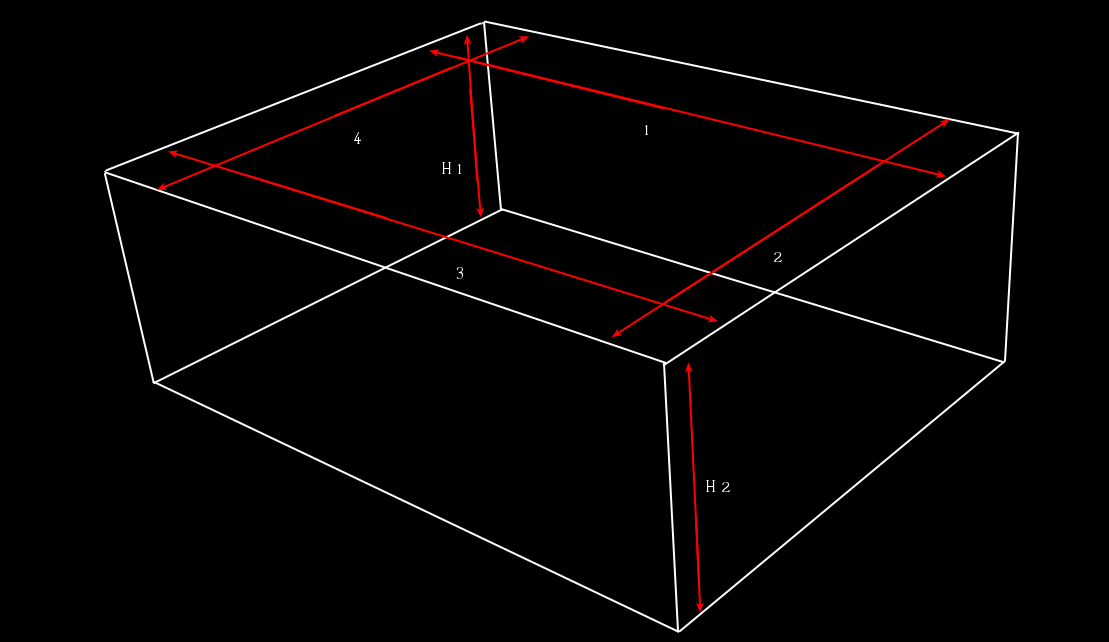
\includegraphics[width=0.7\linewidth]{Includes/images/Results/Selection_013}
			\caption{Locations of the measurements in Table \ref{MeasurmensTable}}
			\label{fig:SourceOfMEasure}
		\end{figure}
		
		\noindent It is important to note that the Oriented bounding box of the room has the dimensions 5.795m, 7.455m, 2.900m. The OBB is therefore 37cm bigger along the width of the room, 25cm in the length and 40cm bigger vertically. This is important because it may look like a bounding box has been created but that is not the case.
		
	\section{Accuracy of resulting model}
		Figure \ref{fig:Planefitingaccuracy} shows how a specific segment varies from the final model. The error ranges from perfect fit, shown in red, to an error of 10mm in the blue section at the top left. 
		
		\begin{figure}[H]
		\centering
		\includegraphics[width=1\linewidth]{"Includes/images/Results/Plane fiting accuracy"}
		\caption{Blue to Red scale of point variance from fitted plane on right hand wall segment }
		\label{fig:Planefitingaccuracy}
		\end{figure}
		
		It is easy to see that the only major deviation from a perfect fit is in the top left of the Figure, this is due to a poster being stuck on the wall there. It is reassuring to see that even with the poster on the wall the results have not been effected.
	
	\section{Limitations of this process}
	\label{Limitations}
		As it stands the main limitations on this process are the complexity of the room that is scanned. Rooms that are reasonably rectangular can be processed successfully. But as soon as small sections start to kink out or there are walls that start to run at different angles the Extrusion method explained in section \ref{Extrusion} fails. This can be seen in the images of a secondary point cloud boundary representation process in Appendix B.
		
	\section{File Size}
	
		A benefit of this system is that large point clouds can be greatly reduced in size without loss of to much vital information. Of coarse there is a loss of detail, but as said in the previous section this is a current limitation on the process, but can be overcome in future versions of this system.
		
		The two indoor scans of around started off with a resolution of 1.3mm point spacing at a distance of 10m, file sizes of around 7GB. Through down sampling the point clouds the point spacing was increased uniformly to a 1cm, reducing file size to less than 50MB. Then after the process outlined is this report is run on the down sampled point cloud they are simplified to 24 points and a file size of under 5KB.
		
		Obviously as the detail in the model increases and materials start to be used the file size will increase but never to the extent that a full point cloud will. 
		

	
\chapter{Conclusions and Future work}

In conclusion this report has succeeded is creating a process to create boundary representations of indoor rooms. The process described in this report is still, however, in its infancy, and has a few limitations.


\section{Improving Detail in the System}

	The progression from the point that this process is at can be extended in a number of directions, firstly the current models created are very simplistic and cannot deal with rooms that have more than 6 sides, essentially only very simple rooms. The need for this process to be able to deal with more complex rooms is the first major improvement that will take place. 
	
	From the complexity of the rooms increasing, the detail in the model is the next step in making the process more complete, adding doors and windows into the models. This presents its own new challenges because the program will need to be able to differentiate between wall segments, door segments and general cluttering segments. This makes the segments selection section substantially more important.
	
\section{Extending the Process to Multiple Rooms}
	
	Another extension to this system is the ability to process more complex networks of rooms. Figure \ref{fig:complexscene} shows a complex network or rooms that could potentially be turned into CAD models in the future of this process. This concept can be extended even further into multiple story networks. From here it becomes necessary to create topology in the points before they are processed, so that rooms and floors can be differentiated from each other.
	
	
	\begin{figure}[htb]
		\centering
		\includegraphics[width=1\linewidth]{"Includes/images/Results/complex scene"}
		\caption{A more complex network of rooms within a building}
		\label{fig:complexscene}
	\end{figure}
	
\section{User Interface}
	Currently the whole system is run from a command line and the parameters are fixed with no way to change them other than recompiling the whole project. Creating a user interface that allows users to change parameters themselves as well as a visualizer build into the user interface that allows users change parameters and see the result in the same window. This is the final step in making this system into a full package,is to build additional, and unrelated, functionality into the system. Such as creating mesh models of point clouds or even simple down sampling of clouds. 
	
	
	